\newpage
\section{Accessible}

The data is considered accessible by the user when he does not need to make an excessive effort to
to be able to obtain them, understand them and use them, that is, apply them to their particular situation. To achieve these objectives,
it is necessary that the user can access them in a way that is familiar and in a language and nomenclature
he can understand.\\ 

So how do we consider that data is accessible to a user?
\begin{itemize}
\item When it is easy to obtain.
The data should be readily available over the web.
\item When it is easy to understand.
The data must be represented in such a way that it's meaning is clear and obvious to a non-specialist. 
Imagine a science writer explaining a complicated concept for a mass market magazine audience. Use everyday language and easily interpretable diagrams.
\item When it is easy to use.
A user must be able to apply the data to their own particular purpose without complicated procedure.
\end{itemize}



In this section we will see if it is possible to access data by an average user and how to optimize accessibility.

\subsection{Disponibilidad}
    
As we mentioned in the introduction to this chapter, the data sets may be available in the original source, but not by
This means that they are accessible.
The challenges that we encounter with the raw data, direct from the source of origin, are the following: \\   
 
\textbf{Location}. Data sets are available in organized open data portals
and structured, you usually need a search and selection task
sometimes complicated. Although companies put more and more of their part in offering an interface
pleasant and functional to users, this task requires a research work by the user,
Since possibly, you should look in different portals. \\

\textbf{Extraction}. Data sets are usually available through a programming interface
of applications (API) not easily interpretable by the average user. Normally has
a document that describes each of the fields and values that are presented in the document and how to use the API. \\

\textbf{Readability}. Usually the data sets are represented in a format to be processed by
some software, so its reading is complicated by the average user, at best,
they will be represented in a table and even then, it will be very difficult to extract information.

Therefore, we can not say that these data are accessible in a useful way for the average user. \\

\subsubsection{How to solve it.} 

We must provide the information required by the user directly, easy to read and interpret. In a format
that is easy and fast to assimilate.

For the correct use of the data we will have to carry out processes such as extraction, transformation and
data cleaning, so you get the data you need to show the useful information.
 
\subsubsection{How we solve it. Aire Guru.} 

Our tool uses the air quality data provided by the city of Malaga in its open data portal.\footnote{\url{https://datosabiertos.malaga.eu/}}\\
\begin{figure}[ht]
    \centering
   \subfigure[Main page]
    {\includegraphics[width=5.5cm  ]{OpenDataPortal}}
    \hfill
    \subfigure [Category environment]
       { \includegraphics[width=5.5cm]{openDataPortalEnviromentCategory}}
    \vfill
     \subfigure[GeoJson Document]
     { \centering \includegraphics[width=4.75cm]{geoJsonAirQualityDataRaw}}
  
  \caption{Open Data Portal Malaga}
    \end{figure}

    This data portal offers an offer of categories represented by icons, so it is necessary to know in which category the set is classified
    of data, once the category is accessed, we have a search bar that allows us to insert the keywords to search the data set
    wanted.\\
    
    In this case you can click on the link and this will open the data in a new tab, so the use of a computer system
    for downloading the data is not strictly necessary, but we can see that the format is not readable, at least from the point
    of human sight.

AireGuru \footnote{\url{https:\\aire.guru}} offers all the necessary information on a web platform with an adapted visualization
to human understanding.
\newpage
\elsparagraph{Evaluation}  

\begin{itemize}
    \done Location. The location of the data is direct, since it offers information from the first moment in which the web is accessed. On the main page
         presents the levels of pollution in all areas without the need to make any selection.
    \done Extraction. No software or computer knowledge is necessary to access the information.
    \done Readability. It contains a map where the pollution levels are presented by colors. These colors are defined by a fair legend
         below the map. It has a glossary that explains the concepts presented on the website, the meaning of each section and how
         browse the web page.
 

\end{itemize}
\newpage

 



\subsection{Know about}

The user will need to know that he has this resource and can use it because although we optimize the represantation of the
data set and we offer it to users, this will not be useful if users are not aware that it exists.

\subsubsection{How to solve it} 
The best way is to advertise the product in the right environment and environment.
\subsubsection{How we solve it. Aire Guru} 
Our tool is implemented for the city of Malaga, so we are currently working to give it to
know in this city.
It is currently available in the open data portal in the app tab \footnote {\url {https://datosabiertos.malaga.eu/aplicaciones}} \\
Participated in the first open data reuse contest organized by the Malaga City Council \footnote {\url {https://tinyurl.com/yx9wzutj}}
being finalist in the category of web page.


\begin{figure}[ht]
    \centering
   \subfigure[Advertising in the open data portal of Málaga]{ \centering \includegraphics[width=6cm]{aireGuruFinalist}}
   \hfill
   \subfigure[Finalist]{ \centering \includegraphics[width=5cm]{aireGuruFinalistCertificate}}
 
    \caption{I Contest of reuse of open data. Malaga's town hall}
    \end{figure}

\elsparagraph{Evaluation}  
\begin{itemize}
    \done It is currently published in the open data portal of the City of Malaga.
\crossed More work should be done on the advertising of the platform and make it known.
\end{itemize}
\newpage
\subsection{Interpretabilidad}
The platforms provide a huge volume of data, since, as mentioned earlier, they collect as much data as possible.
There will be multiple samples containing the specified set of fields. These field sets may be similar to each other but don't need to be identical.
From this data, we need to select the relevant samples, and from these, the fields necessary to represent specific information.


Below we can see examples. The first one is taken from the European open data portal
\footnote{\url{https://tinyurl.com/y3d76525}} and the second from the North American open data portal\footnote{\url{https://data.cityofnewyork.us/api/views/kku6-nxdu/rows.json?accessType=DOWNLOAD}}.

\begin{figure}[h]
    \centering
    \subfigure[EEUU Open Portal.Demographic Statistics By Zip Code]
     {\includegraphics[width=5cm]{ExampleOpenDataEEUU}}
    \hfill
     \subfigure[European Open Data Portal. Air pollutant concentrations 2015]
    {\includegraphics[width=7cm]{ExampleOpenDataEuropean}}
    \caption{Open Data Examples}
\end{figure}

    

    
\subsubsection{How to solve it} 
We obtain our required data through a series of processes such as extraction, transformation and
cleaning of the data. Without automation, theses processes are tedious and time consuming. 

\subsubsection{How we solve it. Aire Guru} 

The extracted data is in GeoJSON format, a format which provides a JSON object with nested subdocuments. Each of these
subdocuments contains a set of data in key form value.
In the following figure we can see the beginning of the document downloaded on June 9, 2019
\footnote{\url{https://datosabiertos.malaga.eu/recursos/ambiente/calidadaire/calidadaire.json}}\\
\newpage
\begin{figure}[h]
    \centering
   \subfigure[First subdocument]{ \centering \includegraphics[width=4.75cm]{geoJsonAirQualityData1}}
   \hfill
   \subfigure[Second subdocument]{ \centering \includegraphics[width=4.75cm]{geoJsonAirQualityData2}}
 
    \caption{Air quality Document [09/06/2019].Open Data Portal Malaga}
    \end{figure}
    
    In this excerpt we can see the first two subdocuments. Each subdocument contains the coordinates of the air quality measuring station, the date and time when the measurement was recorded, and the values of the measurements.
    In the following figure we can find the description provided by the open data portal.
\begin{figure}[ht]
    \centering
    \includegraphics[width=8cm]{geoJsonAirQualityDataDescription}
    \caption{Air quality data description [09/06/2019].Open Data Portal Malaga}
\end{figure}


For a more detailed description of the measures, we have to resort to an external resource. In this case we directly contacted 
the company that installs the UrbanClouds\footnote{\url{https://urbanclouds.city/es/}} measuring stations and provides the data to the Malaga city council.

After selecting the necessary fields according to our design plan, we carried out different cleaning, transformation and extraction tasks. \\


\textbf{Cleaning}. We need to eliminate the repeated or non-relevant fields. For example, the identifier of the measuring station is  unneccessary as the data set already contains the coordinates of the station, and coordinate representation is more interesting for our purposes. \\

\textbf{Transformation}. We need the values to have a format appropriate to the fields that they represent. For example, the date and time of the measurement is stored in date format
instead of the string provided in the raw data set. \\

\textbf{Extraction}. We need to select the relevant fields. This data set offers one or more measurements for each pollutant, which can be represented by three different fields, a
quantitative measurement, a qualitative of the fixed station of measurement and a qualitative station of a mobile station. We will add a field containing the measurement which is most relevant for our purposes, and eliminate the non-relevant measurerments to minimize processing time. \\

For security, a second totally independent architecture has been implemented that collects and stores the raw data.

\paragraph{Evaluation} \mbox{} 
\begin{itemize}
    \done We can understand exactly what each one of the fields represented in the data set means thanks to the information
         complementary information presented in the open data portal and by the complementary information provided by the company in charge of
         collect the data.
    \done The data needed for our model has been extracted from the raw data.
    
\end{itemize}
\newpage

\subsection{Modelo}

Recall that the main objective of accessing the data is to obtain knowledge, to understand and make sense of it. Of course, 
pure data by itself has no value until we can understand it and apply it. We must contextualize, process, and analyze the 
information to gain useful knowledge. \\
    
\begin{figure}[ht]
    \centering 
    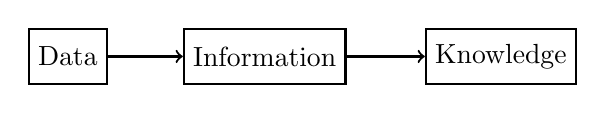
\begin{tikzpicture}[thick]
        \node[draw,rectangle,minimum size=20] (a) {Data};
         \node[draw,rectangle,minimum size=20,right of= a, node distance=2.5cm] (b) {Information};
         \node[draw,rectangle,minimum size=20,right of=b, node distance=3cm] (c) {Knowledge};
         \draw[->] (a) to (b);
        \draw[->] (b) to (c);
     
      \end{tikzpicture}
      \caption{Diagrama. De datos a conocimiento}
    \end{figure}
 
    In order to obtain this knowledge, the user must correctly interpret the data. It's not enough to know what the values and 
    units individually represent, but what they mean in the big picture. For that the user must already have expertise in the 
    area, or must engage in further research allowing them to understand the data that has been extracted.
     
    In order to build a system that makes data accessible, it is essential to design a model to specify the
    information that we want to obtain. The design of a system will allow that, based on given values, provide some results.
    For this it will be necessary to have a solid knowledge of the dataset that is needed, the values,
    their units and how they relate to each other.


\subsubsection{How to solve it} 
Study the objective sought and resort to the help of experts if necessary to acquire the necessary knowledge
on the subject. Design a model that provides the information we are looking for.

\subsubsection{How we solve it. Aire Guru} 
Aire Guru aims to increase the awareness of the level of pollution that surrounds us. To do this, it uses a measure called
the air quality index (AQI), specifically the European air quality index (EAQI).


\newpage
\begin{figure}[ht]
    \centering
    \includegraphics[width=10cm]{mapAireGuru}
    \caption{Aire Guru. Landing page. Top section}
\end{figure}

It shows the AQI in the whole city of Malaga by zones, both the general and the AQI of each of the 
pollutans in a more disaggregated form from September 2018 to the present. It also shows the evolution
of these for days, months and years.
It is capable of creating a set of the most relevant pollutans by medical condition. An innovative feature is the capacity to display levels of any particular pollutant by hour, day, month, or year. 

\elsparagraph{Evaluation}  

\begin{itemize}
\done The information is focused on an objective, informing the user of the level of pollution that surrounds them, both  in real time
and in the past.
\done The information follows a logical thread; it tells a story.
\done The web offers understandabl, useable information, not just raw data.
\end{itemize}

\newpage
\subsection{Formato}
El punto clave para que el usuario entienda lo que queremos transmitirle es crear una comunicacion fluida entre la representacion
de los datos el usuario. Para ello  deberemos asegurarnos que hablamos el mismo idioma, con un vocabulario facil de entender y
con proximidad, es decir,dejar la terminologia a un lado y comunicar el objetivo de la manera mas simple posible.
Por ello la representacion de la informacion jugaran un papel fundamental para que la 
informacion sea absorbida por el usuario de una manera natural.

\textcolor{red}{\textbf{Por Aqui voy}}

El apartado anterior "Interpretabilidad", vimo que un conjunto de datos en crudo no siempre era el mas adecuado para la mayoria de los usuarios.
Deberemos estudiar que tipo de representacion es mas adecuada, no siempre una grafica es la representacion mas adecuada, deberemos hacer un 
estudio de tanto al publico al que va dirigido como como podemos acentuar la informacion que sea mas relevante en la manera 
correcta.
Si nos declinamos por realizar una representacion con graficas, deberemos estudiar los datos para saber que tipo de grafica. Por ejemplo, si hablamos de muestras y queremos saber la 
densidad, nos inclinaremos por un grafico de densidad y si por ejemplo buscamos la diferencia entre sexos, utilizaremos un grafico de tartas.



\subsubsection{How to solve it} 
Este modelo debera proporcional la informacion al usario en un lenguaje o formato compresible. Si no es posible proporcionarmos las herramientas necesarias para que este pueda 
comprender el contexto de la informacion.
Es importante que proporcionemos la informacion en un idioma que el usuario entienda, ya sea este literal o visual.
Hablamos de vocabulario y terminologia, deberemos huir de los tecnicismo que sumerjan al usuario en una nube de 
imcomprensibilidad, ya que

\subsubsection{How we solve it. Aire Guru} 
Nuestra herramienta utiliza como componenete principal un mapa sobre el que se representa el AQI general calculado. Este es un formato 
mas legible para los usuarios. Este indice mustra un indicador con cinco niveles: "Insalubre" "Malo" "Pobre" "Aceptable" y "Bueno" y 
especifica un rango de colores desde el rojo hasta el celeste.\\
Nuestra plataforma introduce ademas una iconografica para ayudar al usuario a tener una idea directa de la situacion, ya que son mas 
explicativos que los colores. En caso de peligro, queda bien representado con el color rojo, pero en el caso del azul o verde, en nuestra cultura, no
tenemos definido un estado para estos colores.\\
\begin{figure}[ht]
    \centering
    \includegraphics[width=12cm]{EAQUI_Icons}
    \caption{Iconografica Aire Guru}
\end{figure}

Ademas proporciona un glosario con las descripciones de los agentes contaminantes, complicaciones medicas, fuentes de contaminacion
y la iconografia utilizada y una ayuda donde se puede consultar el calculo de AQI y ampliar informacion.

La herramienta Aire guru presenta la informacion en el idioma nativo de la ciudad y se utiliza un lenguaje sencillo y directo.
Ademas se utiliza el mismo estilo, colores e iconografia en todo el diseno para que el usuario se familierize rapidamente y pueda
prestar atencion al significado de los datos en vez de perderse en el diseno e intentar encontrar su significado.
 
\elsparagraph{Evaluation}  
\begin{itemize}
    \done El lenguaje utilizado en toda la herramienta es un lenguaje comun, huye de la terminologia cientifica pero proporciona la informacion
    suficiente para enteder la situacion.
    \crossed Algunos terminos especificos no se han podido sustituir como "Indice de calidad del Aire".
    \done Se han proporcionado la herramientas necesarias para entender el concepto. Se ha utilizado la norma europea de calidad del aire para 
    representar los valores y se ofrece al usuario recursos en la pagina para su comprension ademas de recursos extenos.
    
\end{itemize}
 

\newpage
\subsection{Convenience}
As we mentioned earlier, our goal is for the user to have access to the direct data without having to deal with any
of the technical processes involved in implementing a system. The points we must cover to achieve this goal are: \\

\textbf{Infrastructure}. Data collection, processing, storage and visualization. For example, in most cases, the data is
published periodically, but the set of published data only contains the most recent samples, so there is no way to obtain
a history of the data if they are not collected, processed and stored periodically. \\

\textbf{Automation}. As we commented in the previous point, these tasks are repetitive and also tend to be arduous processes, so it will be
necessary to automate it, otherwise the effort required by the user to extract the information will not compensate. \\

\textbf{Availability} To offer data to users in a direct way, it is recommended to use a platform to which the user
be familiar For example, it is more feasible that the user feels more attracted to access the data if it does not require
no installation on your devices. \\

\subsubsection{How to solve it} 
We will have to provide all the mentioned infrastructure to be able to carry out all the steps to complete the path of obtaining the
raw data until offering them to the user in an accessible, relevant and irresistible way.
We will try to free the user from repetitive actions, we will automate all the possible processes, to offer the user the information as soon as possible.
directly possible.
We must offer the information through a platform with which the user is familiar, nowadays the use of websites or mobile applications is very common.
It is advisable to offer all the possible information without having to make the user perform complicated actions and do not require any additional software or hardware.

\subsubsection{How we solve it. Aire Guru} 
Malaga's air quality data set is updated every hour, Aire Guru automates the process of collecting the
data through a CRON job that executes a script implemented in JavaScript periodically. This reads the data from the url, processes them,
clean and store in a MongoDB database. That is to say, it implements all the necessary structure.

Thanks to this infrastructure, the user is able to visualize the evolution of pollutants since 2018. You can also see the exhibition
personal to these pollutant during the same period of time.

In addition, with the automation of processes, the user is able to visualize the pollution in real time of the city of Malaga and specifically in the point
in which it is found. \\

\begin{figure}[ht]
    \centering
    \includegraphics[width=12cm]{aireGuruArquitecture}
    \caption{Arquitecture Aire Guru}
\end{figure}

Mediante una interfaz web, muestra los datos al usuarios.\\

\begin{figure}[ht]
    \centering
    \includegraphics[width=9cm]{aireGuru}
    \caption{Aire Guru. Web Interface}
\end{figure}

To guarantee the reach of the majority of the population, Aire Guru is available at the web addresses https://www.aire.guru and https://www.airquality.guru.
Use SSL that guarantees the encryption of data through the network, more and more browsers try to protect users and
They only show pages that use a secure method.

As we commented previously, all users can see the basic information without having to provide any data or identify themselves, without the need to
perform no download or installation and today, almost everyone is familiar with web browsing.
When we do not force the user to perform extra actions, such as a download or identification, the user will feel less forced to give us an opportunity.


\elsparagraph{Evaluation}  
\begin{itemize}
\done The data necessary for our model have been extracted from the raw data.
\done Infrastructure. It implements all the necessary architecture of storage, processing and visualization so that the user only has to consult
the data.
\done It automates the processes of data collection and the necessary calculations to show the information to the user.
\done Offering users a free web page, facilitates the user to access information directly
\end{itemize}


